\section{Die Deutsche Kreditbank AG}\label{einleitung}

Die Deutsche Kreditbank Aktiengesellschaft ist ein Kreditinstitut mit Sitz in Berlin. Dabei ist Sie eine hundertprozentige Tochtergesellschaft der Bayerischen Landesbank. Das Geschäft der DKB beruht auf zwei Säulen: dem als Direktbank betriebenen Privatkundengeschäft und der Tätigkeit als Geschäftsbank mit Finanzierung- und Anlagelösungen für Kommunen und Unternehmen. Im Jahr 2019 stand die DKB nach Kundenzahlen auf dem zweiten Platz der größten Direktbanken Deutschlands. 
Die DKB wurde als erste private Bank der DDR am 19.03.1990 in Form einer Aktiengesellschaft gegründet und unterhält heute deutschlandweit mehr als 26 Standorte. Das bekannteste Produkt ist das Girokonto „DKB Cash“, wobei es sich um ein reines Online-Konto handelt. Daneben hat die DKB private Immobilienfinanzierungen, Brokerage, Ratenkredite und Sparprodukte im Angebot. Die Bank betreibt nur wenige eigene Geldautomaten, ermöglicht aber eine gebührenfreie Nutzung für den Kunden an Fremdautomaten mit der zum Online-Konto gehörenden VISA-Kreditkarte.

\subsection{DKB Service GmbH}\label{einleitung}
\begin{figure}[H] 
  \centering
     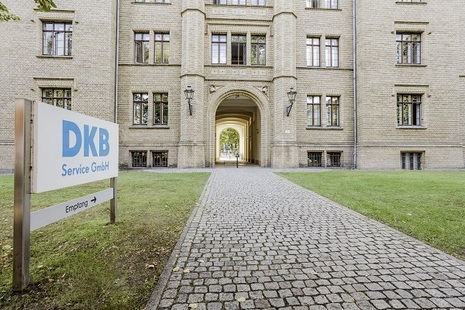
\includegraphics[width=1\textwidth]{dkb.jpg}
  \caption{Hauptsitz in Potsdam}
  \label{fig:Bild1}
\end{figure}
\noindent
Die DKB Service GmbH ist ein hundertprozentiges Tochterunternehmen der DKB AG und hat ihren Hauptsitz in Potsdam bei Berlin. Gegründet wurde sie 2001, ist heute an 17 Standorten vertreten und mit über 1.700 Mitarbeiter*innen der Dienstleistungspartner in der DKB-Gruppe. Dabei bündelt sie Dienstleistungen in folgenden 8 Geschäftsfeldern:

\begin{enumerate}
	\item BankDienstleistungen
	\item CustomerCare
	\item Facility Management
	\item IT-Dienste
	\item Marketing
	\item Finanzen
	\item Human Resources
	\item SAP Business Solutions
\end{enumerate}

\subsection{Geschäftsfeld IT-Dienste}\label{einleitung}


Das Geschäftsfeld IT-Dienste fungiert mit ihren Produkten als erster Ansprechpartner in der DKB-Gruppe mit Sitz in der Herzbergstraße in Berlin Lichtenberg. Das Feld reicht von IT-technischer Ausstattung der Arbeitsplätze inklusive Hard- und Software bis hin zum SAP-Betrieb mit Softwareentwicklung und Anwenderbetreuung. Es wird besonders Wert auf die ganzheitliche IT-technische Betreuung des Kunden*innen gelegt. So begann meine Werkstudententätigkeit in diesem Feld im Team Mobiles Arbeiten. Im Arbeitsalltag bedeutete das ein umfangreiches Portfolio an Aufgaben, welches vom Aufbau und Wartung von Hardware, schreiben von Programmen zur Optimierung von Prozessen oder Umsetzung eigener Projekte, persönlicher Support und  Wiederinstandsetzung der Hardware von Führungskräften oder Versenden der Post ein breites Feld abdeckte.  So wurden dort nicht nur elektrotechnische und informationstechnische, sondern auch körperliche Fähigkeiten gefordert. Das Team Mobiles Arbeiten bestand aus 10 Mitarbeitern und meinem direkten Chef und Leiter des Teams Jan Trotzer. Im Kerngeschäft ging es um die Organisation, Dokumentation, Wartung und den Versandt von IT-technischer Hardware an Mitarbeiter der DKB AG. Als Werkstudent im Bereich Computer Engineering sollte ich die Lücke zwischen den informationstechnischen Anforderungen und den hardwaretechnischen Umsetzungen schließen und versuchen Alltagsprozesse zu optimieren und zu verbessern. So konnte ich das Team nicht nur durch eigene Programmierung, sonder auch durch kleinere Reperaturen und Sicherheit im Umgang mit Computern und Hardware bereichern. 

